\newpage
\noindent
\textbf{Beispiel 2}\\ \\
a)\\ \\
Freigeschnittene Objekte:
\begin{figure}[h]
	\centering
	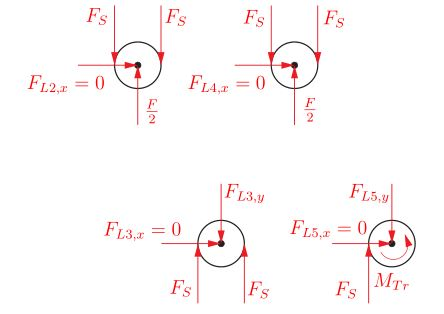
\includegraphics[width= 10cm]{tikz/17_07_2017_2a}
\end{figure}
\newline
Die benötigten Gleichgewichtsgleichungen lauten hier für die erste Umlenkrolle
\begin{align*}
	\textbf{e}_x &: F_{L2,x} = 0 \\
	\textbf{e}_y &: -2F_S + \frac{F}{2} = 0 
\end{align*}
für die zweite Umlenktrommel
\begin{align*}
	\textbf{e}_x &: F_{L3,x} = 0 \\
	\textbf{e}_y &: 2F_S - F_{L3,y} = 0 \\
\end{align*}
für die dritte Umlenkrolle
\begin{align*}
	\textbf{e}_x &: F_{L4,x} = 0\\
	\textbf{e}_y &: -2F_S + \frac{F}{2} = 0 \\
\end{align*}
und für die Trommel
\begin{align*}
	\textbf{e}_x &: F_{L5,x} = 0\\
	\textbf{e}_y &: F_S - F_{L5,y} = 0\\
	\textbf{e}_z &: M_{TR} - F_S\frac{d}{2}
\end{align*}
\newpage
\noindent
b)\\ \\
Um die benötigten Lagerkräfte zu bestimmen muss man nur die Gleichgewichtsgleichungen beachten und entsprechend umformen. Für die Seilkraft folgt aus zweiten Gleichung der ersten Rolle
\[
	F_S = \frac{F}{4}
\]
Daher lauten die Kräfte für das Lager 1 (durch freischneiden von Lager 1)
\begin{align*}
	F_{L1,x} &= 0 \\
	F_{L2,y} &= F_S = \frac{F}{4}
\end{align*}
für das Lager 3
\begin{align*}
	F_{L3,x} &= 0 \\
	F_{L3,y} &= 2F_S = \frac{F}{2}
\end{align*}
und für das Lager 5
\begin{align*}
	F_{L5,x} &= 0 \\ 
	F_{L5,y} &= F_S = \frac{F}{4}
\end{align*}
c)\\ \\
Das Trommelmoment lautet
\[
	M_{TR} = \frac{Fd}{8}
\]
Mit dem Übersetzungsverhältnis aus der Angabe folgt schließlich für das Haltemoment
\[
	M_M = \frac{Fd}{8i}
\]